% ===
%
% Official LaTeX seminar report template of the
% Chair for AI Methodology (AIM)
% RWTH Aachen University, Aachen, Germany
%
% Author: Jakob Bossek (bossek@aim.rwth-aachen.de)
%
% AIM website: https://aim.rwth-aachen.de/
%
% ===

% The 'review' option activates line numbering
\documentclass[review]{AIM_report}

% includes/preamble.tex is the right place to add new packages etc.
% tables
\RequirePackage{booktabs}
\RequirePackage{colortbl}
\RequirePackage{multicol}
\RequirePackage{multirow}
\RequirePackage{xspace}
\RequirePackage[final]{pdfpages}

% \smiley{} and \frowney{}
\RequirePackage{wasysym}

% quotation
\RequirePackage{csquotes}


% import commenting macros
%% commenting macros

% use this to hide larger blocks of material:
\usepackage{xcolor}
\usepackage{amsmath,amssymb}

% Define colors for authors
\definecolor{janecolor}{rgb}{0.2,0.6,0.6}
\definecolor{johncolor}{rgb}{0,0.7,0}

% Define colors for general macros
\definecolor{todocolor}{rgb}{0.9,0.1,0.1}
\definecolor{changedcolor}{rgb}{0.42,0.27,0.57}
\definecolor{addedcolor}{rgb}{0.867,0.176,0.361}

% General comment macro
\newcommand{\nbc}[3]{
    {\colorbox{#3}{\bfseries\sffamily\scriptsize\textcolor{white}{#1}}}
    {\textcolor{#3}{\sf\small$\blacktriangleright$\textit{#2}$\blacktriangleleft$}}
}
  
% Define individual comments for authors
\newcommand{\jane}[1]{\nbc{Jane}{#1}{janecolor}}
\newcommand{\john}[1]{\nbc{John}{#1}{johncolor}}

% Define general helper macros
\newcommand{\todo}[1]{\nbc{TODO}{#1}{todocolor}}
\newcommand{\changed}[1]{\nbc{CHANGED}{#1}{changedcolor}}
\newcommand{\added}[1]{\nbc{ADDED}{#1}{addedcolor}}

\newcommand{\redacted}[1]{\emph{[anonymized for review]}}
%\renewcommand{\redacted}[1]{#1}

% Use this to temporarily hide reviewing comments, todos, etc.:
%  \renewcommand{\jane}[1]{}
%  \renewcommand{\john}[1]{}

% Use this to make "changed" items appear normal:
%\renewcommand{\changed}[1]{#1}
%\renewcommand{\added}[1]{#1}
%\renewcommand{\todo}[1]{}

%% end commenting macros


% metadata
\title{Rapid Time Serires Datasets Library}
\subtitle{Efficient AI with Rust Lab}
\author{Marius Kaufmann (422046) \and Amir Ali Aali (463040) \and Kilian Fin Braun (422030)}

\institute{RWTH Aachen University, Germany\\
\email{$\{$amir.ali.aali, john.doe$\}$@rwth-aachen.de}}

% source file(s) with bibliography entries
\addbibresource{bib.bib}

\begin{document}

\maketitle

\section{Introduction}

We use the \LaTeX{} package \texttt{biblatex} for citations. Sample citation:~\cite{HutterEtAl2009}. You can also use full citations: \fullcite{HBPSTK2021TSPnormalization}

You are free to use British, American, Canadian or Australian English, but whatever you choose should be used consistently.
As Europeans, we recommend the use of British English (which is also well supported by spell and grammar checkers).

\newpage
\pagestyle{empty}

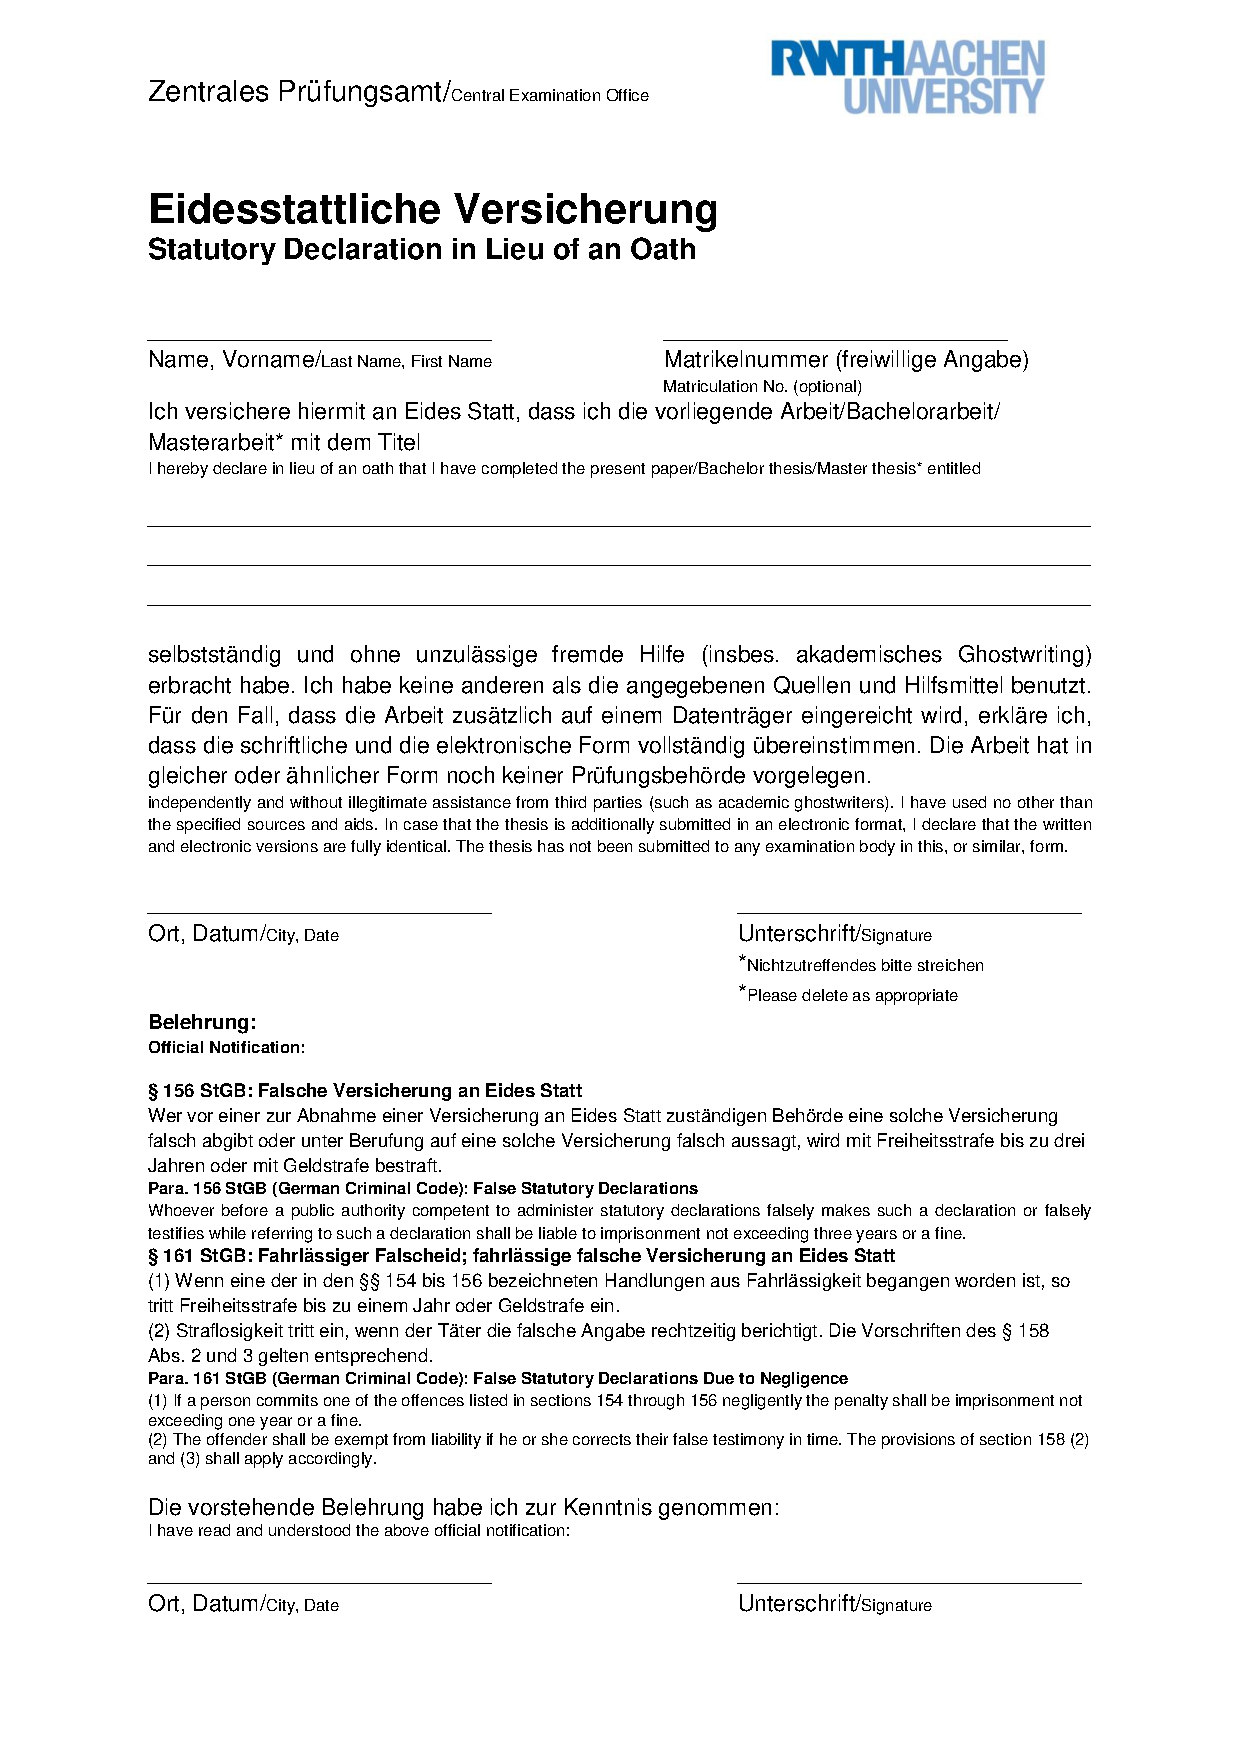
\includepdf[pages=-,pagecommand={},width=\textwidth]{files/oathstatement.pdf}

\newpage
\pagestyle{empty}

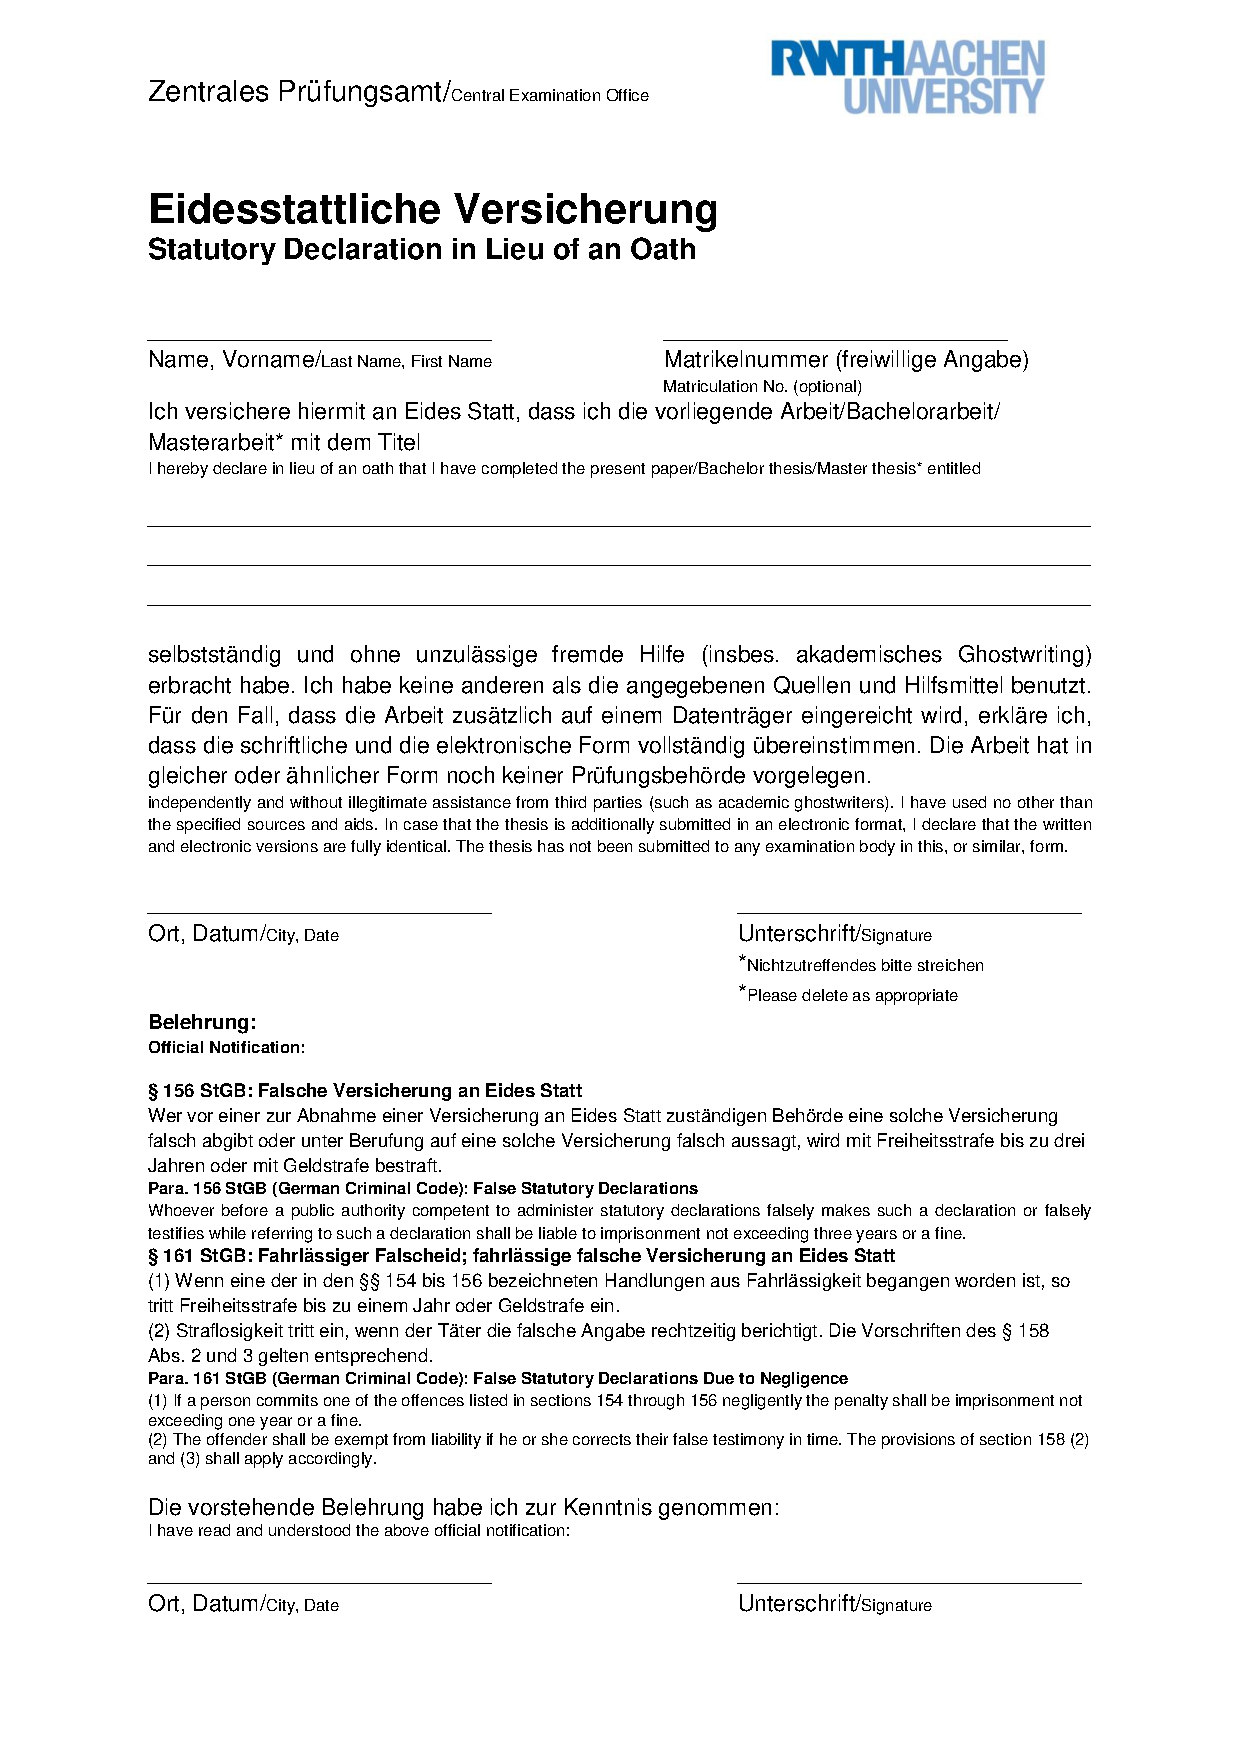
\includepdf[pages=-,pagecommand={},width=\textwidth]{files/oathstatement.pdf}

\newpage
\pagestyle{empty}

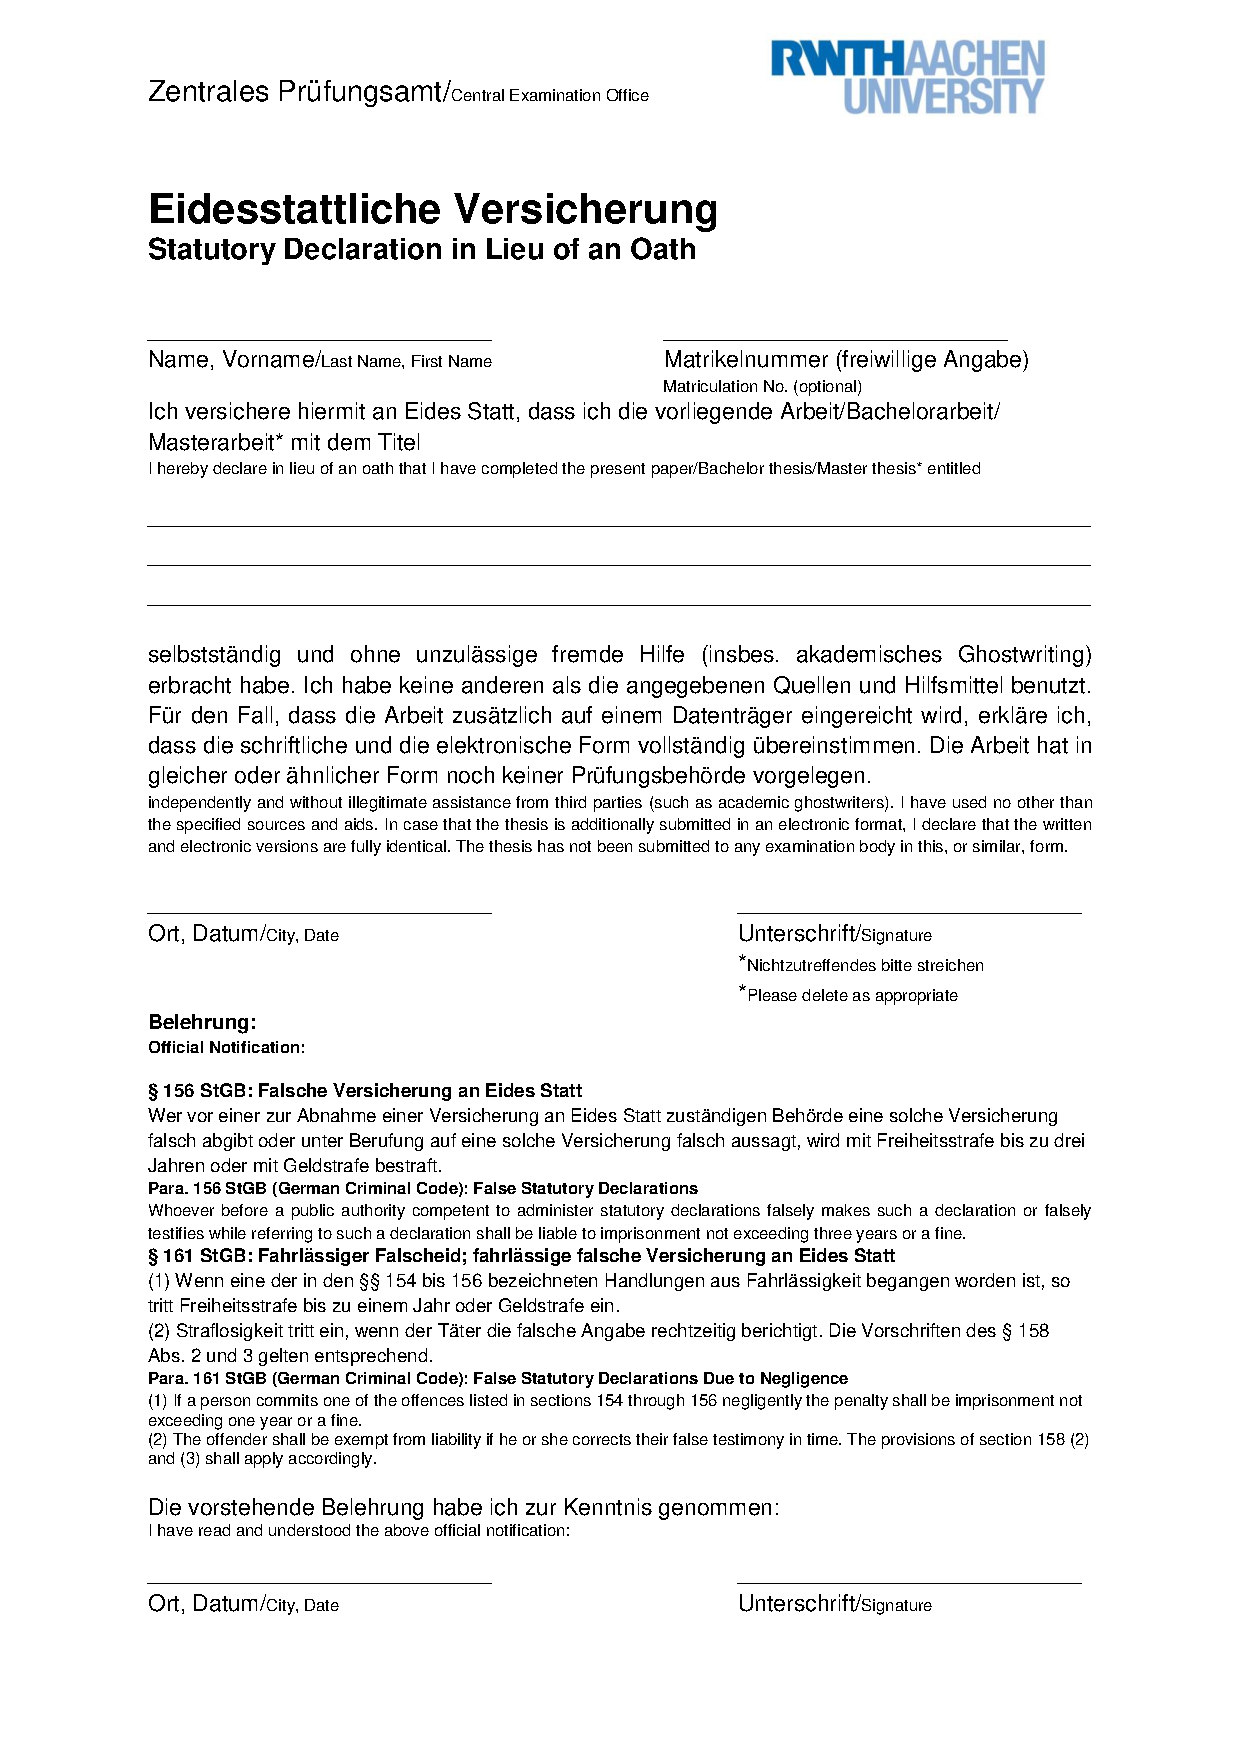
\includepdf[pages=-,pagecommand={},width=\textwidth]{files/oathstatement.pdf}

\end{document}
